\documentclass{beamer}

\mode<presentation>
{
  \usetheme{CambridgeUS}     
  \usecolortheme{default} 
  \usefonttheme{default}  
  \setbeamertemplate{navigation symbols}{}
  \setbeamertemplate{caption}[numbered]
} 
\usepackage{ragged2e}
\usepackage{color}
\usepackage[english]{babel}
\usepackage[utf8x]{inputenc}
\usepackage{graphicx}
\usepackage{tikz} 
\usepackage{array}
\usepackage{amsmath}
\usepackage{booktabs}
\usepackage{multirow}
\usepackage{makecell}
\usepackage{longtable}
\usepackage{varwidth}
\usepackage{threeparttable}
\renewcommand{\raggedright}{\leftskip=0pt \rightskip=0pt plus 0cm}

\title[Growth and Corruption]{Firm Growth and Corruption:\\
       \medskip
       \large Empirical Evidence from Vietnam}

\author[Jie Bai]{}

\institute[]{Jie Bai, Seema Jayachandran, Edmund J. Malesky, and Benjamin A. Olken \\~\\
\medskip
\textit{Working Paper(2016)}}

\date{$28^{\text{th}}$ April 2017}

\begin{document}

%%%%%%%%%%%%%%%%%%%%%%%%%%%%%%%%%%%%%%%%%%%%%%%%%%%%%%%%%%%%%%%%%%%%%%%%%%%%%%%%%%%%%%%%%%%%%%%%

\begin{frame}
  \titlepage
\end{frame}

%%%%%%%%%%%%%%%%%%%%%%%%%%%%%%%%%%%%%%%%%%%%%%%%%%%%%%%%%%%%%%%%%%%%%%%%%%%%%%%%%%%%%%%%%%%%%%%%

%%%%%%%%%%%%%%%%%%%%%%%%%%%%%%%%%%%%%%%%%%%%%%%%%%%%%%%%%%%%%%%%%%%%%%%%%%%%%%%%%%%%%%%%%%%%%%%%
\begin{frame}{Motivation}
\begin{itemize}
\item A striking fact about government corruption is that, no matter how you measure it, it is higher in poor countries.
\end{itemize}
\end{frame}
%%%%%%%%%%%%%%%%%%%%%%%%%%%%%%%%%%%%%%%%%%%%%%%%%%%%%%%%%%%%%%%%%%%%%%%%%%%%%%%%%%%%%%%%%%%%%%%%

%%%%%%%%%%%%%%%%%%%%%%%%%%%%%%%%%%%%%%%%%%%%%%%%%%%%%%%%%%%%%%%%%%%%%%%%%%%%%%%%%%%%%%%%%%%%%%%%
\begin{frame}{Motivation}

\begin{figure}
\centering
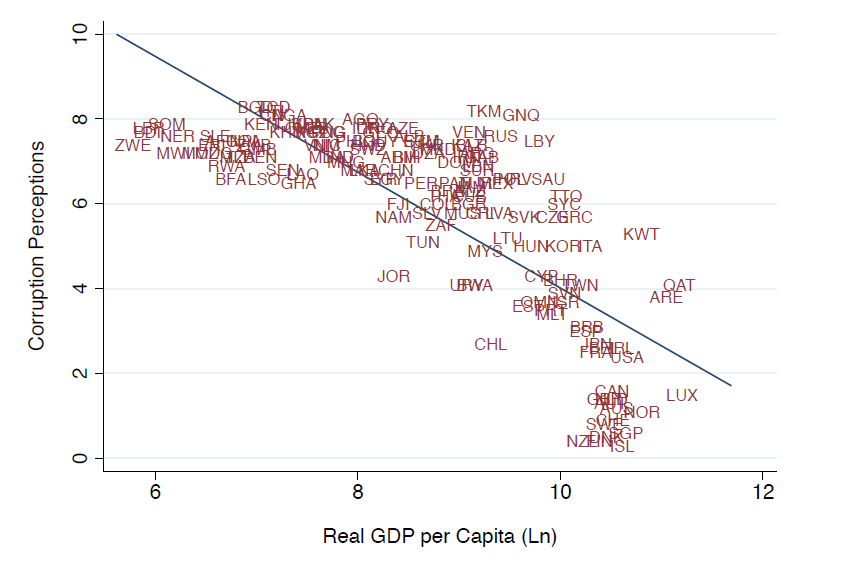
\includegraphics[width=0.8\linewidth]{1.png}
\caption{Transparency International Corruption Index (2005)}
\end{figure}

\end{frame}
%%%%%%%%%%%%%%%%%%%%%%%%%%%%%%%%%%%%%%%%%%%%%%%%%%%%%%%%%%%%%%%%%%%%%%%%%%%%%%%%%%%%%%%%%%%%%%%%

%%%%%%%%%%%%%%%%%%%%%%%%%%%%%%%%%%%%%%%%%%%%%%%%%%%%%%%%%%%%%%%%%%%%%%%%%%%%%%%%%%%%%%%%%%%%%%%%
\begin{frame}{Motivation}

\begin{figure}
\centering
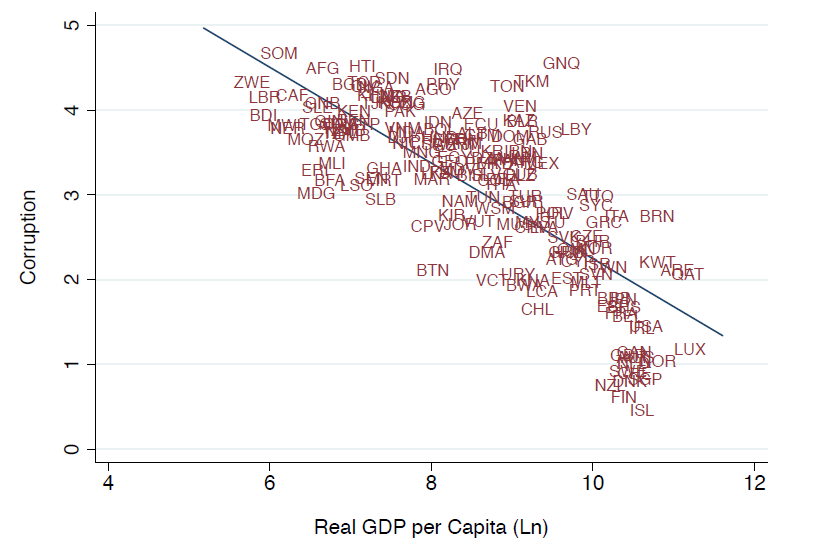
\includegraphics[width=0.8\linewidth]{2.png}
\caption{World Bank Control of Corruption (2005)}
\end{figure}

\end{frame}
%%%%%%%%%%%%%%%%%%%%%%%%%%%%%%%%%%%%%%%%%%%%%%%%%%%%%%%%%%%%%%%%%%%%%%%%%%%%%%%%%%%%%%%%%%%%%%%%

%%%%%%%%%%%%%%%%%%%%%%%%%%%%%%%%%%%%%%%%%%%%%%%%%%%%%%%%%%%%%%%%%%%%%%%%%%%%%%%%%%%%%%%%%%%%%%%%
\begin{frame}{Motivation}

\begin{figure}
\centering
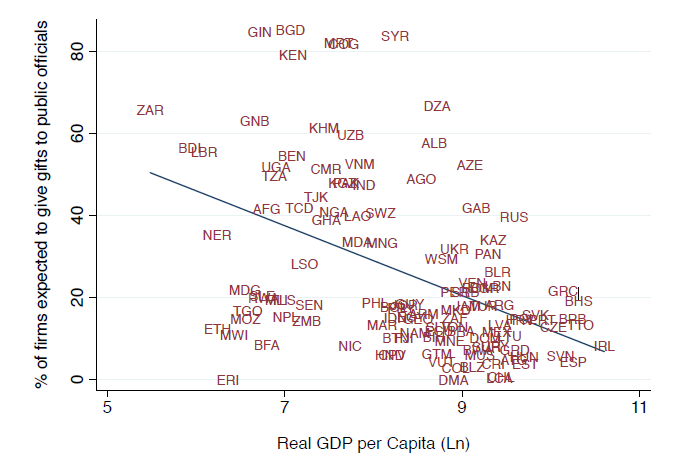
\includegraphics[width=0.8\linewidth]{3.png}
\caption{Relationship Between GDP and Corruption Using Survey Data from Firms}
\end{figure}

\end{frame}
%%%%%%%%%%%%%%%%%%%%%%%%%%%%%%%%%%%%%%%%%%%%%%%%%%%%%%%%%%%%%%%%%%%%%%%%%%%%%%%%%%%%%%%%%%%%%%%%

%%%%%%%%%%%%%%%%%%%%%%%%%%%%%%%%%%%%%%%%%%%%%%%%%%%%%%%%%%%%%%%%%%%%%%%%%%%%%%%%%%%%%%%%%%%%%%%%
\begin{frame}{Motivation}

\begin{itemize}
\item A striking fact about government corruption is that, no matter how you measure it, it is higher in poor countries. \\~
\item While there is a general consensus about the cross-sectional facts, we know relatively little about why corruption is lower in rich countries.
\end{itemize}

\end{frame}
%%%%%%%%%%%%%%%%%%%%%%%%%%%%%%%%%%%%%%%%%%%%%%%%%%%%%%%%%%%%%%%%%%%%%%%%%%%%%%%%%%%%%%%%%%%%%%%%

%%%%%%%%%%%%%%%%%%%%%%%%%%%%%%%%%%%%%%%%%%%%%%%%%%%%%%%%%%%%%%%%%%%%%%%%%%%%%%%%%%%%%%%%%%%%%%%%
\begin{frame}{Prior Work}

\begin{itemize}
\item One hypothesis is that the pattern reflects a negative causal effect of corruption on economic growth:Corruption discourages investment which, in turn, depresses growth.[Mauro, 1995; Wei, 1999a] \\~

\item The correlation might also be due to the reverse causal link: Economic growth could reduce corruption, so as countries grow, corruption naturally declines.[Huntington, 2002; Bardhan, 1997; Glaeser and Goldin, 2004]
\begin{itemize}
\item Evidence for a causal link between growth and reduced corruption has not been definitively established.
\item The mechanisms by which growth reduces corruption are poorly understood.
\end{itemize}

\end{itemize}

\end{frame}
%%%%%%%%%%%%%%%%%%%%%%%%%%%%%%%%%%%%%%%%%%%%%%%%%%%%%%%%%%%%%%%%%%%%%%%%%%%%%%%%%%%%%%%%%%%%%%%%

%%%%%%%%%%%%%%%%%%%%%%%%%%%%%%%%%%%%%%%%%%%%%%%%%%%%%%%%%%%%%%%%%%%%%%%%%%%%%%%%%%%%%%%%%%%%%%%%
\begin{frame}{Overview}
\begin{itemize}
\item This paper studies the link from growth to reduced corruption, aiming to improve on the causal identification in the existing literature.

\begin{itemize}
\item Focus on one dimension of growth,firm growth; one form of corruption, namely bribes extracted from
firms by government officials; and one country, Vietnam. \\~
\end{itemize}

\item Establishes two empirical facts:
\begin{enumerate}
\item Economic growth reduces the proportion of firm revenues extracted by government officials as bribes.
\item This reduction in corruption is larger for firms that can more easily relocate.
\end{enumerate}

\end{itemize}

\end{frame}
%%%%%%%%%%%%%%%%%%%%%%%%%%%%%%%%%%%%%%%%%%%%%%%%%%%%%%%%%%%%%%%%%%%%%%%%%%%%%%%%%%%%%%%%%%%%%%%%

%%%%%%%%%%%%%%%%%%%%%%%%%%%%%%%%%%%%%%%%%%%%%%%%%%%%%%%%%%%%%%%%%%%%%%%%%%%%%%%%%%%%%%%%%%%%%%%%
\begin{frame}

\frametitle{Outline}
\tableofcontents

\end{frame}
%%%%%%%%%%%%%%%%%%%%%%%%%%%%%%%%%%%%%%%%%%%%%%%%%%%%%%%%%%%%%%%%%%%%%%%%%%%%%%%%%%%%%%%%%%%%%%%%

%%%%%%%%%%%%%%%%%%%%%%%%%%%%%%%%%%%%%%%%%%%%%%%%%%%%%%%%%%%%%%%%%%%%%%%%%%%%%%%%%%%%%%%%%%%%%%%%
\section{Data and Institutional Background}
%%%%%%%%%%%%%%%%%%%%%%%%%%%%%%%%%%%%%%%%%%%%%%%%%%%%%%%%%%%%%%%%%%%%%%%%%%%%%%%%%%%%%%%%%%%%%%%%

%%%%%%%%%%%%%%%%%%%%%%%%%%%%%%%%%%%%%%%%%%%%%%%%%%%%%%%%%%%%%%%%%%%%%%%%%%%%%%%%%%%%%%%%%%%%%%%%
\begin{frame}{Background on Vietnam}

\begin{itemize}
\item At its 6th Party Congress in 1986, the country initiated the Doi Moi (Renovation) economic reforms, which eliminated the role of central planning in the economy and opened the country's borders to international capital and trade flows(Riedel and Turley, 1999).\\~
\item Three post-Doi Moi events are also critical for understanding Vietnam's economic development in the period we study.
\begin{enumerate}
\item The Enterprise Law in 2000 created the formal legal basis for the private.
\item Vietnam finalized the long standing negotiations with the United States over their bilateral trade agreement (US-VN BTA).
\item Vietnam joined the World Trade Organization in 2007.\\~
\end{enumerate}

\item The degree of economic growth over this period varied considerably across provinces.
\end{itemize}

\end{frame}
%%%%%%%%%%%%%%%%%%%%%%%%%%%%%%%%%%%%%%%%%%%%%%%%%%%%%%%%%%%%%%%%%%%%%%%%%%%%%%%%%%%%%%%%%%%%%%%%

%%%%%%%%%%%%%%%%%%%%%%%%%%%%%%%%%%%%%%%%%%%%%%%%%%%%%%%%%%%%%%%%%%%%%%%%%%%%%%%%%%%%%%%%%%%%%%%%
\begin{frame}{Background on Vietnam}

\begin{itemize}
\item Despite this growth, there is still substantial corruption in Vietnam. \\~
\item Existing research has noted that corruption in Vietnam takes three main forms(Vasavakul,2008).
\begin{enumerate}
\item Grease or speed money to fulfill basic tasks or services
\item Illegal privatization of state property 
\item Selling of state power \\~
\end{enumerate}
\item An important institutional feature of Vietnam is that corruption is largely subnational.
\begin{itemize}
\item The provincial leadership has the ability to control the bribe schedule of the province both directly and indirectly.
\end{itemize}

\end{itemize}

\end{frame}
%%%%%%%%%%%%%%%%%%%%%%%%%%%%%%%%%%%%%%%%%%%%%%%%%%%%%%%%%%%%%%%%%%%%%%%%%%%%%%%%%%%%%%%%%%%%%%%%

%%%%%%%%%%%%%%%%%%%%%%%%%%%%%%%%%%%%%%%%%%%%%%%%%%%%%%%%%%%%%%%%%%%%%%%%%%%%%%%%%%%%%%%%%%%%%%%%
\begin{frame}{Background on Vietnam}

\begin{figure}
\centering
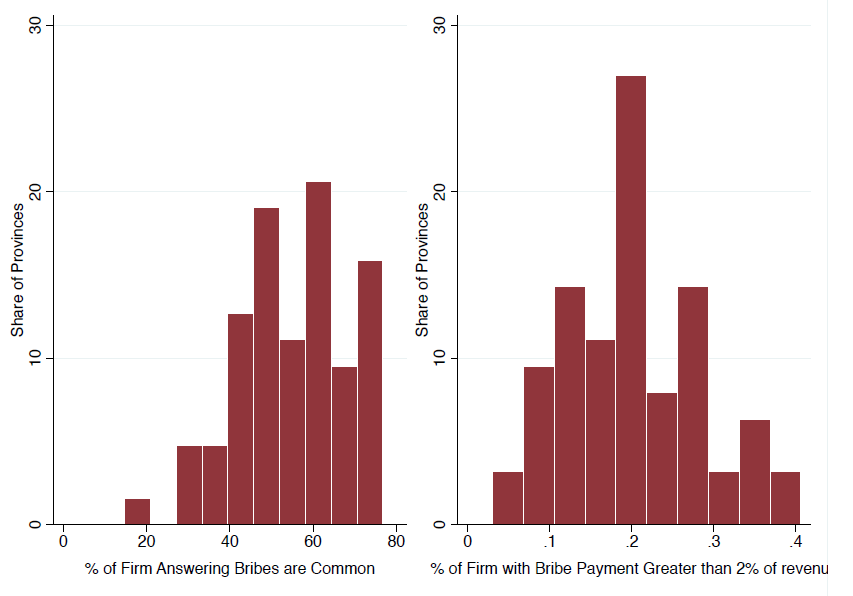
\includegraphics[width=0.8\linewidth]{4.png}
\caption{Variation in Corruption across Provinces in Vietnam}
\end{figure}

\end{frame}
%%%%%%%%%%%%%%%%%%%%%%%%%%%%%%%%%%%%%%%%%%%%%%%%%%%%%%%%%%%%%%%%%%%%%%%%%%%%%%%%%%%%%%%%%%%%%%%%

%%%%%%%%%%%%%%%%%%%%%%%%%%%%%%%%%%%%%%%%%%%%%%%%%%%%%%%%%%%%%%%%%%%%%%%%%%%%%%%%%%%%%%%%%%%%%%%%
\begin{frame}{Description of data}
\begin{itemize}
\item Two firm-level data sets from Vietnam 
\begin{enumerate}
\item Vietnam PCI Survey(Malesky, 2011),contains basic firm-level information,including the firm's ISIC 2 digit industry code, location(province), year of establishment, total assets, and total employment.
\item Annual enterprise survey collected by the General Statistics Office of Vietnam. \\~
\end{enumerate}

\item Aggregate employment data at the industry from the Chinese Yearbook of Labor Statistics \\~

\item Five years of repeated cross-sectional firm-level data from 2006 to 2010.

\end{itemize}

\end{frame}
%%%%%%%%%%%%%%%%%%%%%%%%%%%%%%%%%%%%%%%%%%%%%%%%%%%%%%%%%%%%%%%%%%%%%%%%%%%%%%%%%%%%%%%%%%%%%%%%

%%%%%%%%%%%%%%%%%%%%%%%%%%%%%%%%%%%%%%%%%%%%%%%%%%%%%%%%%%%%%%%%%%%%%%%%%%%%%%%%%%%%%%%%%%%%%%%%
\begin{frame}{Description of data}

\begin{figure}
\centering
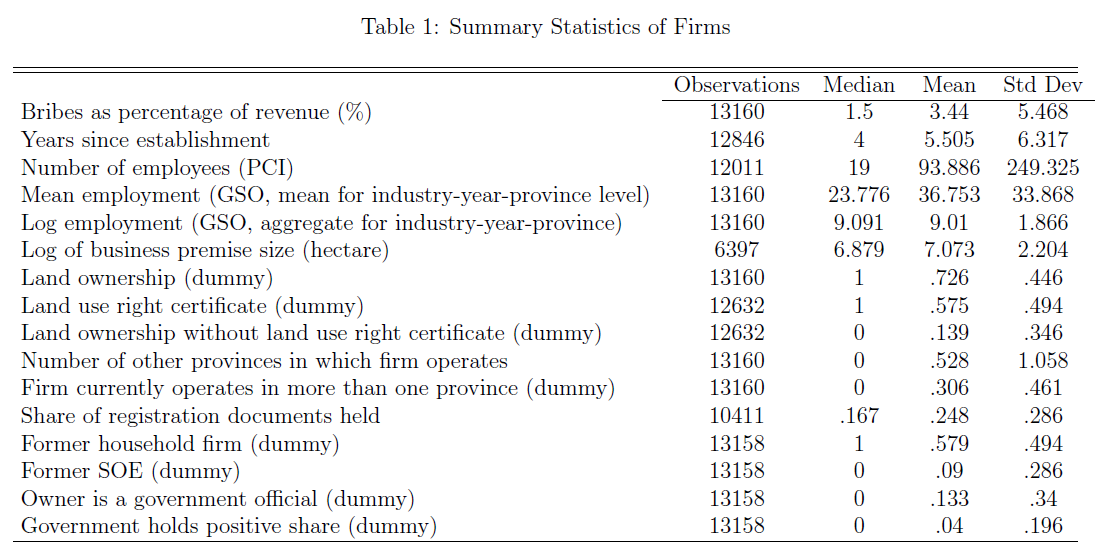
\includegraphics[width=1\linewidth]{5.png}
\end{figure}

\end{frame}
%%%%%%%%%%%%%%%%%%%%%%%%%%%%%%%%%%%%%%%%%%%%%%%%%%%%%%%%%%%%%%%%%%%%%%%%%%%%%%%%%%%%%%%%%%%%%%%%

%%%%%%%%%%%%%%%%%%%%%%%%%%%%%%%%%%%%%%%%%%%%%%%%%%%%%%%%%%%%%%%%%%%%%%%%%%%%%%%%%%%%%%%%%%%%%%%%
\begin{frame}{Description of data}

\begin{itemize}
\item The key dependent variable is constructed from the PCI question that asks the firm its unofficial payments as a percentage of total revenue.
\begin{itemize}
\item The question is categorical, with the following possible responses: 0,$<$1\%,1-2\%,2-10\%,10-20\%,20-30\%,$>$30\%.
\end{itemize}

\end{itemize}

\end{frame}
%%%%%%%%%%%%%%%%%%%%%%%%%%%%%%%%%%%%%%%%%%%%%%%%%%%%%%%%%%%%%%%%%%%%%%%%%%%%%%%%%%%%%%%%%%%%%%%%

%%%%%%%%%%%%%%%%%%%%%%%%%%%%%%%%%%%%%%%%%%%%%%%%%%%%%%%%%%%%%%%%%%%%%%%%%%%%%%%%%%%%%%%%%%%%%%%%
\begin{frame}{Description of data}

\begin{figure}
\centering
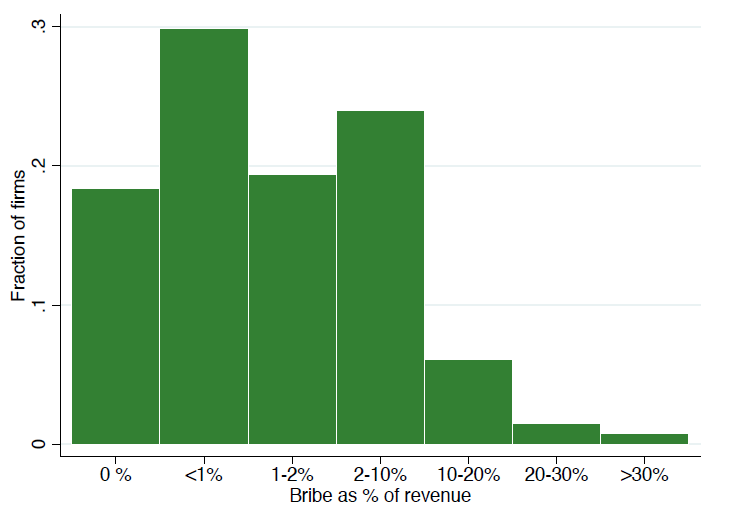
\includegraphics[width=0.8\linewidth]{6.png}
\caption{Histogram of Bribe Rate}
\end{figure}

\end{frame}
%%%%%%%%%%%%%%%%%%%%%%%%%%%%%%%%%%%%%%%%%%%%%%%%%%%%%%%%%%%%%%%%%%%%%%%%%%%%%%%%%%%%%%%%%%%%%%%%

%%%%%%%%%%%%%%%%%%%%%%%%%%%%%%%%%%%%%%%%%%%%%%%%%%%%%%%%%%%%%%%%%%%%%%%%%%%%%%%%%%%%%%%%%%%%%%%%
\begin{frame}{Description of data}

\begin{itemize}
\item The key dependent variable is constructed from the PCI question that asks the firm its unofficial payments as a percentage of total revenue.
\begin{itemize}
\item The question is categorical, with the following possible responses: 0,$<$1\%,1-2\%,2-10\%,10-20\%,20-30\%,$>$30\%. \\~
\end{itemize}

\item Transform the variable into a scalar by assigning each response the middle of the corresponding bin, using 0.5\% for the $<$ 1\% category and 35\% for the $>$ 30\% category.\\~

\item Also consider an alternative specification using ordered probit models that allows the model to determine appropriate breakpoints,results are similar.

\end{itemize}

\end{frame}
%%%%%%%%%%%%%%%%%%%%%%%%%%%%%%%%%%%%%%%%%%%%%%%%%%%%%%%%%%%%%%%%%%%%%%%%%%%%%%%%%%%%%%%%%%%%%%%%

%%%%%%%%%%%%%%%%%%%%%%%%%%%%%%%%%%%%%%%%%%%%%%%%%%%%%%%%%%%%%%%%%%%%%%%%%%%%%%%%%%%%%%%%%%%%%%%%
\begin{frame}{Description of data}

\begin{itemize}
\item Our empirical strategy uses aggregate shocks to a firm's industry size as a predictor of the firm's size.
\begin{itemize}
\item Since the PCI is a sample, not a census, to measure the total employment in an industry in each year, we use the annual GSO census of firms in Vietnam to construct industry size.\\~
\end{itemize}

\item Two IVs
\begin{enumerate}
\item Use the GSO data to construct the rest-of-Vietnam IV
\item Use the China Labor Statistical Yearbook to construct China IV
\end{enumerate}

\end{itemize}

\end{frame}
%%%%%%%%%%%%%%%%%%%%%%%%%%%%%%%%%%%%%%%%%%%%%%%%%%%%%%%%%%%%%%%%%%%%%%%%%%%%%%%%%%%%%%%%%%%%%%%%

%%%%%%%%%%%%%%%%%%%%%%%%%%%%%%%%%%%%%%%%%%%%%%%%%%%%%%%%%%%%%%%%%%%%%%%%%%%%%%%%%%%%%%%%%%%%%%%%
\begin{frame}{Description of data}

\begin{figure}
\centering
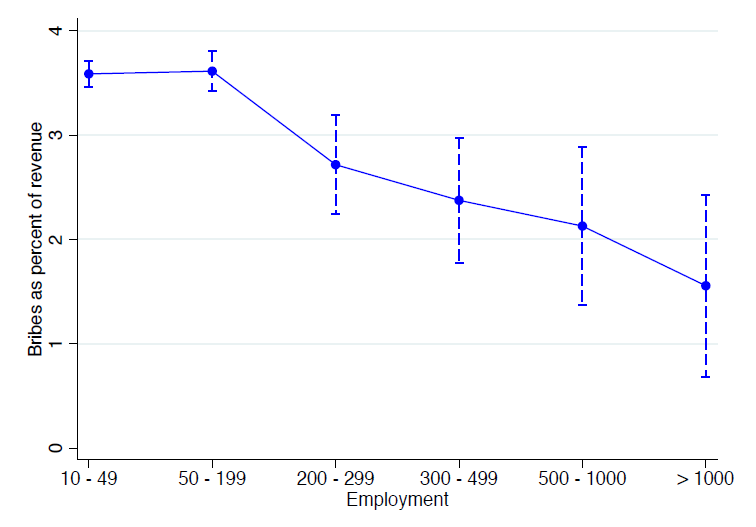
\includegraphics[width=0.8\linewidth]{7.png}
\caption{Cross-Sectional Relationship Between Bribe Rate and Firm Employment}
\end{figure}

\end{frame}
%%%%%%%%%%%%%%%%%%%%%%%%%%%%%%%%%%%%%%%%%%%%%%%%%%%%%%%%%%%%%%%%%%%%%%%%%%%%%%%%%%%%%%%%%%%%%%%%

%%%%%%%%%%%%%%%%%%%%%%%%%%%%%%%%%%%%%%%%%%%%%%%%%%%%%%%%%%%%%%%%%%%%%%%%%%%%%%%%%%%%%%%%%%%%%%%%
\section{Empirical Strategy}
%%%%%%%%%%%%%%%%%%%%%%%%%%%%%%%%%%%%%%%%%%%%%%%%%%%%%%%%%%%%%%%%%%%%%%%%%%%%%%%%%%%%%%%%%%%%%%%%

%%%%%%%%%%%%%%%%%%%%%%%%%%%%%%%%%%%%%%%%%%%%%%%%%%%%%%%%%%%%%%%%%%%%%%%%%%%%%%%%%%%%%%%%%%%%%%%%
\begin{frame}{Empirical strategy}
\begin{itemize}
\item The hypothesis we aim to test is that firm growth has a negative effect on bribes. \\~
\item With data on firms indexed by i in province p, industry j,and time t, one could in principle test the hypothesis via OLS as follows:
\begin{equation}
Bribes_{ipjt}=\alpha +\beta A_{ipjt}+\epsilon _{ipjt}
\end{equation}

\item Two issues with estimating Equation (1) directly:
\begin{itemize}
\item Data problem: we do not directly observe TFP or output prices in the data, so, empirically,we use rm employment (Employ) as a proxy.Under the assumption that factor prices are constant, changes in employment reflect changes in A.(show later)
\item Employment levels are potentially endogenous to the bribe level b. Thus, we estimate Equation (1) via two IV strategies.
\end{itemize}

\end{itemize}

\end{frame}	
%%%%%%%%%%%%%%%%%%%%%%%%%%%%%%%%%%%%%%%%%%%%%%%%%%%%%%%%%%%%%%%%%%%%%%%%%%%%%%%%%%%%%%%%%%%%%%%%

%%%%%%%%%%%%%%%%%%%%%%%%%%%%%%%%%%%%%%%%%%%%%%%%%%%%%%%%%%%%%%%%%%%%%%%%%%%%%%%%%%%%%%%%%%%%%%%%
\begin{frame}{Rest-of-Vietnam IV}

\begin{itemize}
\item The first instrumental variable strategy we use is employment in the firm's industry in Vietnamese provinces other than its own.\\~
\begin{itemize}
\item The IV strategy is predicated on industry-specific employment (or TFP) shocks in an industry being similar across provinces.\\~
\item The identification assumption is that industry-specific bribe-setting is determined independently by each province. 

\end{itemize}

\end{itemize}

\end{frame}	
%%%%%%%%%%%%%%%%%%%%%%%%%%%%%%%%%%%%%%%%%%%%%%%%%%%%%%%%%%%%%%%%%%%%%%%%%%%%%%%%%%%%%%%%%%%%%%%%

%%%%%%%%%%%%%%%%%%%%%%%%%%%%%%%%%%%%%%%%%%%%%%%%%%%%%%%%%%%%%%%%%%%%%%%%%%%%%%%%%%%%%%%%%%%%%%%%
\begin{frame}{Rest-of-Vietnam IV}

\begin{enumerate}
\item Using the leave-one-out Vietnam IV is as follows:
\begin{equation}
\log \left( Employ_{pjt} \right) =\alpha +\beta \log \left( Employ_{p^-jt} \right) +\nu _{pj}+u_t+\epsilon _{pjt} 
\end{equation} \\~

\item The corresponding second stage equation is: 
\begin{equation}
Bribes_{ipjt}=\alpha ^\prime+\beta ^\prime\log \left( \widehat{Employ_{pjt}} \right) +\nu_{pj}^{\prime}+u_{t}^{\prime}+\epsilon _{ipjt}^{\prime}   
\end{equation}

\end{enumerate}

\end{frame}	
%%%%%%%%%%%%%%%%%%%%%%%%%%%%%%%%%%%%%%%%%%%%%%%%%%%%%%%%%%%%%%%%%%%%%%%%%%%%%%%%%%%%%%%%%%%%%%%

%%%%%%%%%%%%%%%%%%%%%%%%%%%%%%%%%%%%%%%%%%%%%%%%%%%%%%%%%%%%%%%%%%%%%%%%%%%%%%%%%%%%%%%%%%%%%%%
\begin{frame}{China IV}

\begin{itemize}
\item One potential concern with the rest-of-Vietnam IV is that it could be correlated with common industry-year specific shocks that affect both firm growth and bribe payments,such as a time-specific national regulatory changes or a national industry-specific crack-down on corruption. \\~

\item Instrument using employment in China.
\begin{itemize}
\item The idea is that many industries in Vietnam and China are subject to the same global business cycles and price and technology shocks, and hence industry-level growth is correlated across the two countries.
\item Because China is so much larger than Vietnam, it is unlikely that there would be reverse causation where changes in a particular industry's corruption level in Vietnam would substantially aect employment growth in China.
\end{itemize}

\end{itemize}

\end{frame}	
%%%%%%%%%%%%%%%%%%%%%%%%%%%%%%%%%%%%%%%%%%%%%%%%%%%%%%%%%%%%%%%%%%%%%%%%%%%%%%%%%%%%%%%%%%%%%%%

%%%%%%%%%%%%%%%%%%%%%%%%%%%%%%%%%%%%%%%%%%%%%%%%%%%%%%%%%%%%%%%%%%%%%%%%%%%%%%%%%%%%%%%%%%%%%%%
\begin{frame}{China IV}

\begin{itemize}
\item One potential concern with the rest-of-Vietnam IV is that it could be correlated with common industry-year specific shocks that affect both firm growth and bribe payments,such as a time-specific national regulatory changes or a national industry-specific crack-down on corruption. \\~

\item Instrument using employment in China. \\~

\item Estimate the following first-stage regression:
\begin{equation}
\log \left( Employ_{pjt} \right) =\alpha +\beta \log \left( EmployChina_{jt} \right) +\nu _{pj}+u_t+\epsilon _{pjt}
\end{equation}

\end{itemize}

\end{frame}	
%%%%%%%%%%%%%%%%%%%%%%%%%%%%%%%%%%%%%%%%%%%%%%%%%%%%%%%%%%%%%%%%%%%%%%%%%%%%%%%%%%%%%%%%%%%%%%%

%%%%%%%%%%%%%%%%%%%%%%%%%%%%%%%%%%%%%%%%%%%%%%%%%%%%%%%%%%%%%%%%%%%%%%%%%%%%%%%%%%%%%%%%%%%%%%%
\begin{frame}{Multiple IVs}

\begin{itemize}
\item The first stage equations described above constrain the effect of a shock to A or Employ in the rest of Vietnam to be the same across industries, and, similarly, the effect of a shock to an industry in China on Vietnamese firms to be the same across industries.\\~

\item Some industries can have positively correlated growth rates between provinces in Vietnam or between China and Vietnam,and some industries can have negatively correlated growth rates.\\~

\item We also allow the first stage coefficients to vary by industry.
\begin{equation}
\log \left( Employ_{pjt} \right) =\alpha +\beta _j\log \left( EmployChina_{jt} \right) +\nu _{pj}+u_t+\epsilon _{pjt}
\end{equation}

\end{itemize}

\end{frame}	
%%%%%%%%%%%%%%%%%%%%%%%%%%%%%%%%%%%%%%%%%%%%%%%%%%%%%%%%%%%%%%%%%%%%%%%%%%%%%%%%%%%%%%%%%%%%%%%

%%%%%%%%%%%%%%%%%%%%%%%%%%%%%%%%%%%%%%%%%%%%%%%%%%%%%%%%%%%%%%%%%%%%%%%%%%%%%%%%%%%%%%%%%%%%%%%
\section{Empirical Results}
%%%%%%%%%%%%%%%%%%%%%%%%%%%%%%%%%%%%%%%%%%%%%%%%%%%%%%%%%%%%%%%%%%%%%%%%%%%%%%%%%%%%%%%%%%%%%%%

%%%%%%%%%%%%%%%%%%%%%%%%%%%%%%%%%%%%%%%%%%%%%%%%%%%%%%%%%%%%%%%%%%%%%%%%%%%%%%%%%%%%%%%%%%%%%%%
\begin{frame}{First stage results}

\begin{figure}
\centering
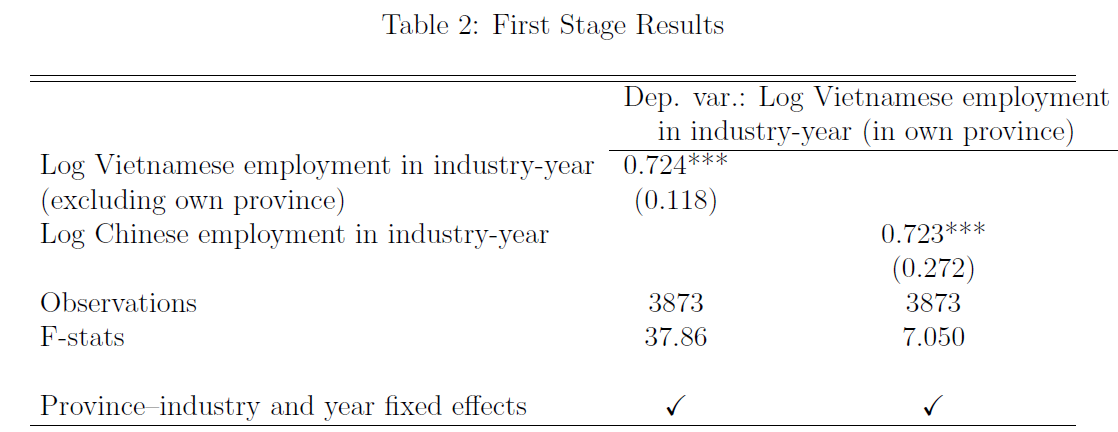
\includegraphics[width=1\linewidth]{8.png}
\end{figure}

\end{frame}
%%%%%%%%%%%%%%%%%%%%%%%%%%%%%%%%%%%%%%%%%%%%%%%%%%%%%%%%%%%%%%%%%%%%%%%%%%%%%%%%%%%%%%%%%%%%%%%

%%%%%%%%%%%%%%%%%%%%%%%%%%%%%%%%%%%%%%%%%%%%%%%%%%%%%%%%%%%%%%%%%%%%%%%%%%%%%%%%%%%%%%%%%%%%%%%
\begin{frame}{First stage results}

\begin{figure}
\centering
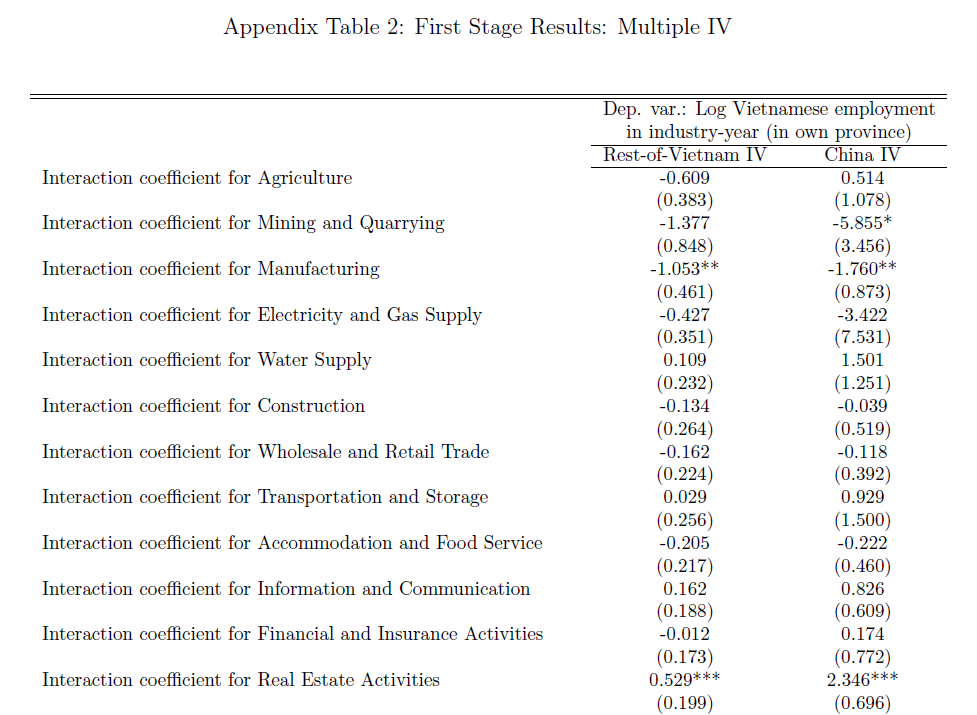
\includegraphics[width=1\linewidth]{9-1.png}
\end{figure}

\end{frame}
%%%%%%%%%%%%%%%%%%%%%%%%%%%%%%%%%%%%%%%%%%%%%%%%%%%%%%%%%%%%%%%%%%%%%%%%%%%%%%%%%%%%%%%%%%%%%%%

%%%%%%%%%%%%%%%%%%%%%%%%%%%%%%%%%%%%%%%%%%%%%%%%%%%%%%%%%%%%%%%%%%%%%%%%%%%%%%%%%%%%%%%%%%%%%%%
\begin{frame}{First stage results}

\begin{figure}
\centering
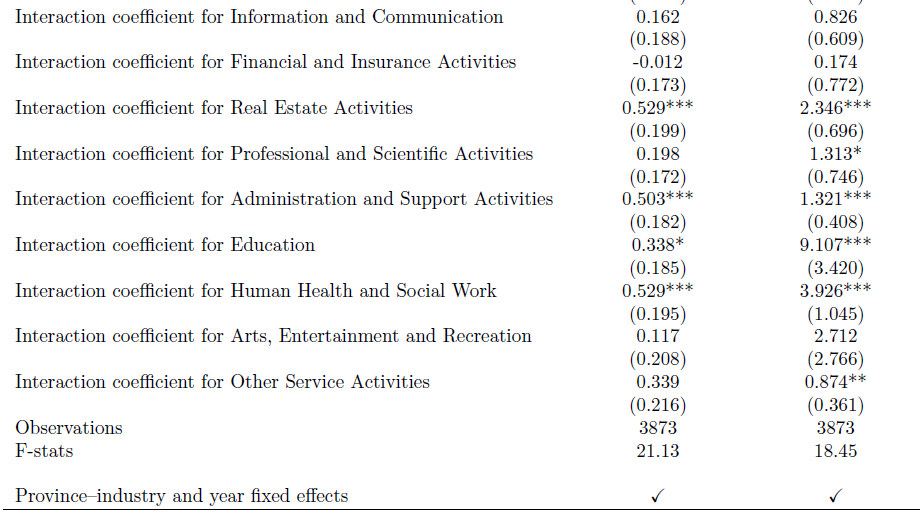
\includegraphics[width=1\linewidth]{9-2.png}
\end{figure}

\end{frame}
%%%%%%%%%%%%%%%%%%%%%%%%%%%%%%%%%%%%%%%%%%%%%%%%%%%%%%%%%%%%%%%%%%%%%%%%%%%%%%%%%%%%%%%%%%%%%%%

%%%%%%%%%%%%%%%%%%%%%%%%%%%%%%%%%%%%%%%%%%%%%%%%%%%%%%%%%%%%%%%%%%%%%%%%%%%%%%%%%%%%%%%%%%%%%%%
\begin{frame}{Validation of matching between PCI and GSO data sets}

\begin{itemize}
\item While the PCI is suitable for examining how a typical firm changes, we cannot use it for accurately calculating aggregate shocks.
\begin{itemize}
\item For example, an increase in prices for goods sold by industry j (one source of an increase in A) might
lead to entry of firms, so even though A increased, average firm size might decrease. \\~
\end{itemize}

\item For this reason, we use the GSO data, which is a census, to construct our measure of A.

\end{itemize}

\end{frame}
%%%%%%%%%%%%%%%%%%%%%%%%%%%%%%%%%%%%%%%%%%%%%%%%%%%%%%%%%%%%%%%%%%%%%%%%%%%%%%%%%%%%%%%%%%%%%%%

%%%%%%%%%%%%%%%%%%%%%%%%%%%%%%%%%%%%%%%%%%%%%%%%%%%%%%%%%%%%%%%%%%%%%%%%%%%%%%%%%%%%%%%%%%%%%%%
\begin{frame}{Validation of matching between PCI and GSO data sets}

\begin{figure}
\centering
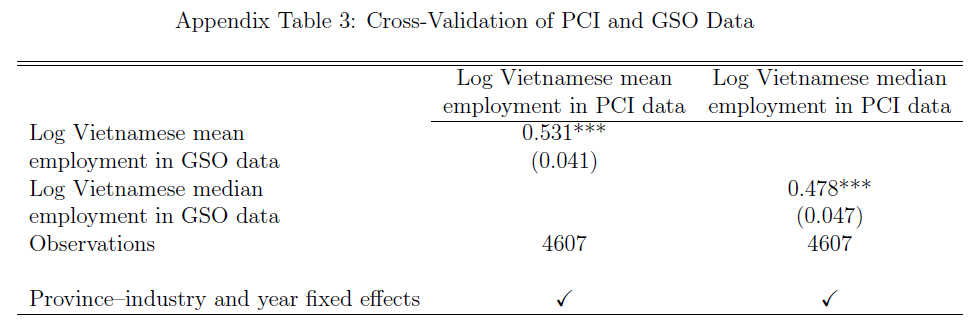
\includegraphics[width=1\linewidth]{10.png}
\end{figure}

\end{frame}
%%%%%%%%%%%%%%%%%%%%%%%%%%%%%%%%%%%%%%%%%%%%%%%%%%%%%%%%%%%%%%%%%%%%%%%%%%%%%%%%%%%%%%%%%%%%%%%

%%%%%%%%%%%%%%%%%%%%%%%%%%%%%%%%%%%%%%%%%%%%%%%%%%%%%%%%%%%%%%%%%%%%%%%%%%%%%%%%%%%%%%%%%%%%%%%
\begin{frame}{Effect of employment growth on bribes}

\begin{figure}
\centering
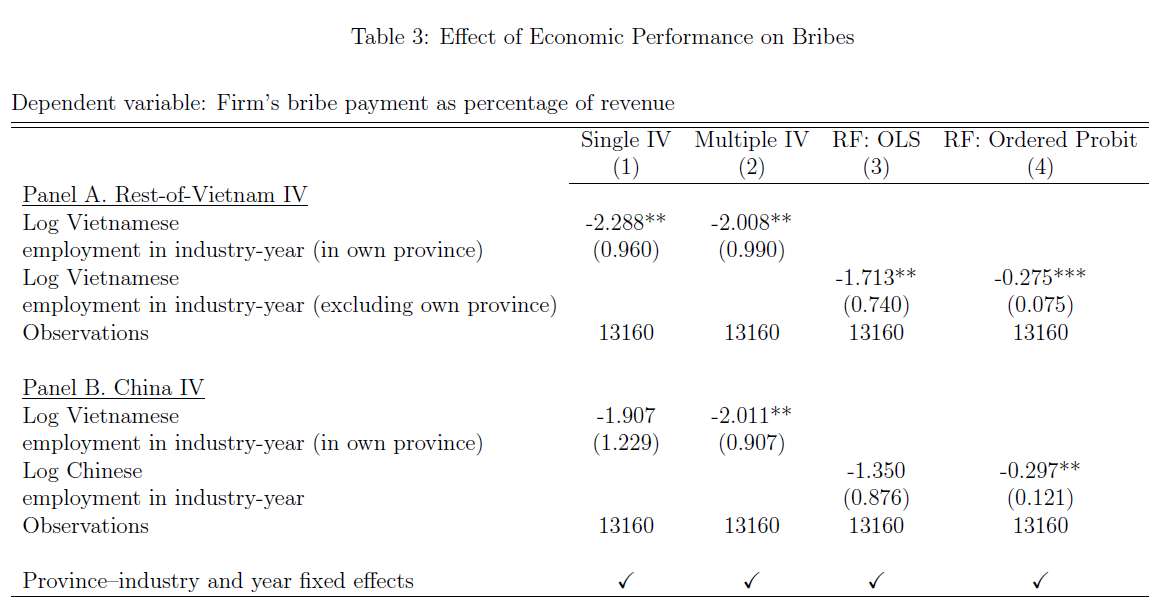
\includegraphics[width=1\linewidth]{11.png}
\end{figure}

\end{frame}
%%%%%%%%%%%%%%%%%%%%%%%%%%%%%%%%%%%%%%%%%%%%%%%%%%%%%%%%%%%%%%%%%%%%%%%%%%%%%%%%%%%%%%%%%%%%%%%

%%%%%%%%%%%%%%%%%%%%%%%%%%%%%%%%%%%%%%%%%%%%%%%%%%%%%%%%%%%%%%%%%%%%%%%%%%%%%%%%%%%%%%%%%%%%%%%
\begin{frame}{Effect of employment growth on bribes}
\begin{itemize}
\item To interpret magnitudes
\begin{itemize}
\item Column 1 implies that a doubling of total employment in the industry is associated with a 1.6 percentage point reduction in informal payments.
\item Translated into an elasticity, this suggests an elasticity of the informal payment rate with respect to predicted firm size of about -0.68.\\~
\end{itemize}

\item The fact that bribes as a share of revenue falls, but the absolute level of bribes rises.

\end{itemize}

\end{frame}
%%%%%%%%%%%%%%%%%%%%%%%%%%%%%%%%%%%%%%%%%%%%%%%%%%%%%%%%%%%%%%%%%%%%%%%%%%%%%%%%%%%%%%%%%%%%%%%

%%%%%%%%%%%%%%%%%%%%%%%%%%%%%%%%%%%%%%%%%%%%%%%%%%%%%%%%%%%%%%%%%%%%%%%%%%%%%%%%%%%%%%%%%%%%%%%
\section{Model}
%%%%%%%%%%%%%%%%%%%%%%%%%%%%%%%%%%%%%%%%%%%%%%%%%%%%%%%%%%%%%%%%%%%%%%%%%%%%%%%%%%%%%%%%%%%%%%%

%%%%%%%%%%%%%%%%%%%%%%%%%%%%%%%%%%%%%%%%%%%%%%%%%%%%%%%%%%%%%%%%%%%%%%%%%%%%%%%%%%%%%%%%%%%%%%%
\begin{frame}{Description}

\begin{itemize}
\item Two subjects
\begin{itemize}
\item Governments choose how much to extract from firms to maximize their bribe revenue.
\item For firms, a bribe is an additional payment to government, analogous to a tax.\\~
\end{itemize}

\item ASSUME 

\begin{itemize}
\item There are two provinces, denoted 1 and 2.Each province is endowed with a unit mass of incumbent firms.
\item All firms have the same two-factor Cobb-Douglas production function with diminishing returns to scale.
\item Capital and labor are perfectly elastically supplied at the same wage rate w and interest rate r in both provinces.
\end{itemize}

\end{itemize}

\end{frame}
%%%%%%%%%%%%%%%%%%%%%%%%%%%%%%%%%%%%%%%%%%%%%%%%%%%%%%%%%%%%%%%%%%%%%%%%%%%%%%%%%%%%%%%%%%%%%%%

%%%%%%%%%%%%%%%%%%%%%%%%%%%%%%%%%%%%%%%%%%%%%%%%%%%%%%%%%%%%%%%%%%%%%%%%%%%%%%%%%%%%%%%%%%%%%%%
\begin{frame}{Description}

\begin{itemize}
\item Government and firms play a static game and move sequentially.\\~
\begin{enumerate}
\item Government in each province p sets a bribe rate $b_p$, which is the percent of a firm's revenues that it must pay in bribes.\\~
\item Firms in each province choose whether to stay in the province or relocate to the other province.\\~
\item Firms choose their factors of production, they produce, and the government collects bribes.
\end{enumerate}

\end{itemize}

\end{frame}
%%%%%%%%%%%%%%%%%%%%%%%%%%%%%%%%%%%%%%%%%%%%%%%%%%%%%%%%%%%%%%%%%%%%%%%%%%%%%%%%%%%%%%%%%%%%%%%

%%%%%%%%%%%%%%%%%%%%%%%%%%%%%%%%%%%%%%%%%%%%%%%%%%%%%%%%%%%%%%%%%%%%%%%%%%%%%%%%%%%%%%%%%%%%%%%
\begin{frame}{Set up}

\begin{itemize}
\item A typical firm in province 1 solves(naturally the analysis is symmetric for firms in province 2)

\begin{equation}
\underset{K\geqslant 0,L\geqslant 0}{\max}\left( 1-b_1 \right) AK^{\alpha}L^{\beta}-wL-rK
\end{equation}

\begin{itemize}
\item Where A is the total factor productivity of the firm. We can also think of A as encompassing the price of the products in the firm's industry.
\end{itemize}

\end{itemize}

\end{frame}
%%%%%%%%%%%%%%%%%%%%%%%%%%%%%%%%%%%%%%%%%%%%%%%%%%%%%%%%%%%%%%%%%%%%%%%%%%%%%%%%%%%%%%%%%%%%%%%

%%%%%%%%%%%%%%%%%%%%%%%%%%%%%%%%%%%%%%%%%%%%%%%%%%%%%%%%%%%%%%%%%%%%%%%%%%%%%%%%%%%%%%%%%%%%%%%
\begin{frame}{Set up and solving}
\begin{itemize}
\item A typical firm in province 1 solves(naturally the analysis is symmetric for firms in province 2)
\begin{equation}
\underset{K\geqslant 0,L\geqslant 0}{\max}\left( 1-b_1 \right) AK^{\alpha}L^{\beta}-wL-rK
\end{equation}
\item This maximization problem yields the following familiar results:

\begin{align}
\frac{L^*}{K^*} & =\frac{r}{w}\frac{\beta}{\alpha}  \\
K^* & =\left( \frac{r}{\left( 1-b_1 \right) A\alpha}\left( \frac{r}{w}\frac{\beta}{\alpha} \right) ^{-\beta} \right) ^{\frac{1}{\alpha +\beta -1}} \\
\pi ^* & = \left( 1-b_1 \right) AK^{*\alpha}L^{*\beta}-wL^*-rK^*
\end{align}

\end{itemize}
\end{frame}
%%%%%%%%%%%%%%%%%%%%%%%%%%%%%%%%%%%%%%%%%%%%%%%%%%%%%%%%%%%%%%%%%%%%%%%%%%%%%%%%%%%%%%%%%%%%%%%

%%%%%%%%%%%%%%%%%%%%%%%%%%%%%%%%%%%%%%%%%%%%%%%%%%%%%%%%%%%%%%%%%%%%%%%%%%%%%%%%%%%%%%%%%%%%%%%
\begin{frame}{Set up and solving}

\begin{itemize}
\item The firm will choose to stay in province 1 if and only if profits in province 1 are greater than profits in province 2 less moving costs, i.e. if $\pi _{f1}^{*}\geqslant \pi _{f2}^{*}-m $, where m is the firm's moving costs.\\~

\item We specify the moving costs for firm i as
\begin{equation}
m_i=\theta A^{\eta}\epsilon _i
\end{equation}

\begin{itemize}
\item The term $A^{\eta}$ captures the fact that the moving costs should be increasing in firm size.
\item The exponent  $\eta$  captures the degree to which moving costs are increasing in the size of the firm.

\end{itemize}

\end{itemize}

\end{frame}
%%%%%%%%%%%%%%%%%%%%%%%%%%%%%%%%%%%%%%%%%%%%%%%%%%%%%%%%%%%%%%%%%%%%%%%%%%%%%%%%%%%%%%%%%%%%%%%

%%%%%%%%%%%%%%%%%%%%%%%%%%%%%%%%%%%%%%%%%%%%%%%%%%%%%%%%%%%%%%%%%%%%%%%%%%%%%%%%%%%%%%%%%%%%%%%
\begin{frame}{Set up and solving}

\begin{itemize}
\item The firm will choose to stay in province 1 if and only if profits in province 1 are greater than profits in province 2 less moving costs, i.e. if $\pi _{f1}^{*}\geqslant \pi _{f2}^{*}-m $, where m is the firm's moving costs.\\~

\item We specify the moving costs for firm i as
\begin{equation*}
m_i=\theta A^{\eta}\epsilon _i
\end{equation*}

\begin{itemize}
\item The $\theta$ term captures the part of the firm's moving costs that is observable to the government.In our empirical analysis, we focus on a firm's property rights status and whether it has operations in multiple provinces
as proxies for the observable components of its moving costs.
\item Moving costs include a stochastic term $\epsilon$ that varies across firms.

\end{itemize}

\end{itemize}

\end{frame}
%%%%%%%%%%%%%%%%%%%%%%%%%%%%%%%%%%%%%%%%%%%%%%%%%%%%%%%%%%%%%%%%%%%%%%%%%%%%%%%%%%%%%%%%%%%%%%%

%%%%%%%%%%%%%%%%%%%%%%%%%%%%%%%%%%%%%%%%%%%%%%%%%%%%%%%%%%%%%%%%%%%%%%%%%%%%%%%%%%%%%%%%%%%%%%%
\begin{frame}{Set up and solving}

\begin{itemize}
\item A firm in province 1 chooses to stay if and only if
\begin{align}
\pi _{1}^{*} & \geqslant \pi _{2}^{*}-\theta A^{\eta}\epsilon ,\ \ or  \\
\epsilon & \geqslant \frac{\pi _{2}^{*}-\pi _{1}^{*}}{\theta A^{\eta}}
\end{align}

\item To simplify the algebra, we further assume that  $\epsilon$ is uniformly distributed over[0,1].
\item The equilibrium number of firms for a given  in province 1 is therefore simply $1-\frac{\pi _{2}^{*}-\pi _{1}^{*}}{\theta A^{\eta}}$
\begin{itemize}
\item This expression will be greater than 1 if $ b_1<b_2 $,and less than 1 if  $ b_1>b_2 $.
\end{itemize}

\end{itemize}

\end{frame}
%%%%%%%%%%%%%%%%%%%%%%%%%%%%%%%%%%%%%%%%%%%%%%%%%%%%%%%%%%%%%%%%%%%%%%%%%%%%%%%%%%%%%%%%%%%%%%%

%%%%%%%%%%%%%%%%%%%%%%%%%%%%%%%%%%%%%%%%%%%%%%%%%%%%%%%%%%%%%%%%%%%%%%%%%%%%%%%%%%%%%%%%%%%%%%%
\begin{frame}{Set up and solving}

\begin{itemize}
\item The two governments in period 1 set bribe rates, taking firms' response and the other province's bribe rate as given.we consider the government in province 1.
\begin{equation}
\underset{b_1\geqslant 0}{\max}b_1AK^{*\alpha}L^{*\beta}\left( 1-\frac{\pi _{2}^{*}-\pi _{1}^{*}}{\theta A^{\eta}} \right) 
\end{equation}     \\~

\item Assuming a symmetric equilibrium($b_{1}^{*}=b_{2}^{*}$), the first-order condition can be simplified to:
\begin{equation}
K^*+b_{1}^{*}\left( \alpha +\beta \right) \frac{dK^*}{db_1}+\frac{b_{1}^{*}K^*}{\theta A^{\eta}}\frac{d\pi _{1}^{*}}{db_1}=0
\end{equation}

\end{itemize}

\end{frame}
%%%%%%%%%%%%%%%%%%%%%%%%%%%%%%%%%%%%%%%%%%%%%%%%%%%%%%%%%%%%%%%%%%%%%%%%%%%%%%%%%%%%%%%%%%%%%%%

%%%%%%%%%%%%%%%%%%%%%%%%%%%%%%%%%%%%%%%%%%%%%%%%%%%%%%%%%%%%%%%%%%%%%%%%%%%%%%%%%%%%%%%%%%%%%%%
\begin{frame}{Set up and solving}

\begin{itemize}
\item The two governments in period 1 set bribe rates, taking firms' response and the other province's bribe rate as given.we consider the government in province 1.
\begin{equation*}
\underset{b_1\geqslant 0}{\max}b_1AK^{*\alpha}L^{*\beta}\left( 1-\frac{\pi _{2}^{*}-\pi _{1}^{*}}{\theta A^{\eta}} \right) 
\end{equation*}     \\~

\item After some algebra, we get:
\begin{equation}
\left( \frac{1}{\theta}A^{1-\eta}\left( \frac{r\beta}{w\alpha} \right) ^{\beta}K^{*\alpha +\beta}+\frac{\alpha +\beta}{1-\alpha -\beta}\frac{1}{1-b^*} \right) b^*=1
\end{equation}

\end{itemize}

\end{frame}
%%%%%%%%%%%%%%%%%%%%%%%%%%%%%%%%%%%%%%%%%%%%%%%%%%%%%%%%%%%%%%%%%%%%%%%%%%%%%%%%%%%%%%%%%%%%%%%

%%%%%%%%%%%%%%%%%%%%%%%%%%%%%%%%%%%%%%%%%%%%%%%%%%%%%%%%%%%%%%%%%%%%%%%%%%%%%%%%%%%%%%%%%%%%%%%
\begin{frame}{Set up and solving}

\begin{itemize}
\item The two governments in period 1 set bribe rates, taking firms' response and the other province's bribe rate as given.we consider the government in province 1.
\begin{equation*}
\underset{b_1\geqslant 0}{\max}b_1AK^{*\alpha}L^{*\beta}\left( 1-\frac{\pi _{2}^{*}-\pi _{1}^{*}}{\theta A^{\eta}} \right) 
\end{equation*}     \\~

\item Several aspects of the equilibrium condition are worth noting.
\begin{enumerate}
\item As $\theta $ goes to $+\infty $ or firms are completely immobile, the expression simplifies such that $b^*=1-\alpha -\beta$.This implies that the greater the diminishing returns to scale, the higher the bribe rate.
\item As $\theta$ decreases, so that moving costs decrease, interregional competition increases and the equilibrium bribe rate decreases.

\end{enumerate}

\end{itemize}

\end{frame}
%%%%%%%%%%%%%%%%%%%%%%%%%%%%%%%%%%%%%%%%%%%%%%%%%%%%%%%%%%%%%%%%%%%%%%%%%%%%%%%%%%%%%%%%%%%%%%%

%%%%%%%%%%%%%%%%%%%%%%%%%%%%%%%%%%%%%%%%%%%%%%%%%%%%%%%%%%%%%%%%%%%%%%%%%%%%%%%%%%%%%%%%%%%%%%%
\begin{frame}{Set up and solving}

\begin{itemize}
\item We examine how the equilibrium bribe rate responds to increases in the profitability of firms, i.e. increases in A. \\~
\item Taking the derivative with respect to logA on both sides of Equation (14) and rearranging terms, we get our first result: \\~

\begin{block}{\ \ \ \ \ \ Proposition 1}
$$
\frac{db^*}{d\log A}<0\ if\ 0\le \eta \le \frac{1}{1-\alpha -\beta}; 
$$
$$
=0\ if\ \eta =\frac{1}{1-\alpha -\beta};and\ >0\ if\ \eta >\frac{1}{1-\alpha -\beta}.
$$
\end{block}

\end{itemize}

\end{frame}
%%%%%%%%%%%%%%%%%%%%%%%%%%%%%%%%%%%%%%%%%%%%%%%%%%%%%%%%%%%%%%%%%%%%%%%%%%%%%%%%%%%%%%%%%%%%%%%

%%%%%%%%%%%%%%%%%%%%%%%%%%%%%%%%%%%%%%%%%%%%%%%%%%%%%%%%%%%%%%%%%%%%%%%%%%%%%%%%%%%%%%%%%%%%%%%
\begin{frame}{Proposition 1}

\begin{itemize}
\item The critical factor that determines the sign of $\dfrac{db^*}{d\log A}$ is $\eta$, which characterizes
the concavity of the moving costs with respect to the capital stock.
\begin{itemize}
\item With a positive shock to A, for a given size, firms enjoy higher revenues and hence care more about the bribes they will pay and less about the moving costs. This tends to drive down the equilibrium bribe rate due to inter-regional competition.
\item However,at the same time, the cost of moving rises as firms expand in size to take advantage of the higher productivity.
\end{itemize}

\end{itemize}

\end{frame}
%%%%%%%%%%%%%%%%%%%%%%%%%%%%%%%%%%%%%%%%%%%%%%%%%%%%%%%%%%%%%%%%%%%%%%%%%%%%%%%%%%%%%%%%%%%%%%%

%%%%%%%%%%%%%%%%%%%%%%%%%%%%%%%%%%%%%%%%%%%%%%%%%%%%%%%%%%%%%%%%%%%%%%%%%%%%%%%%%%%%%%%%%%%%%%%
\begin{frame}{Proposition 1}
\begin{itemize}
\item The critical factor that determines the sign of $\dfrac{db^*}{d\log A}$ is $\eta$, which characterizes
the concavity of the moving costs with respect to the capital stock.
\begin{itemize}
\item Given that $1-\alpha -\beta <1$ a sufficient condition for  $\dfrac{db^*}{d\log A}<0$ is that moving costs scale up less than linearly with rm size, as proxied by A.\\~
\item Moving costs seem likely to fulfill this assumption in practice and, moreover,because $1-\alpha -\beta$ can in fact be much less than 1,it seems plausible that $\eta <\frac{1}{1-\alpha -\beta}$ and therefore  $\dfrac{db^*}{d\log A}<0$ in most settings.

\end{itemize}

\end{itemize}
\end{frame}
%%%%%%%%%%%%%%%%%%%%%%%%%%%%%%%%%%%%%%%%%%%%%%%%%%%%%%%%%%%%%%%%%%%%%%%%%%%%%%%%%%%%%%%%%%%%%%%

%%%%%%%%%%%%%%%%%%%%%%%%%%%%%%%%%%%%%%%%%%%%%%%%%%%%%%%%%%%%%%%%%%%%%%%%%%%%%%%%%%%%%%%%%%%%%%%
\begin{frame}{Set up and solving}

\begin{itemize}
\item We examine how the equilibrium bribe rate responds to increases in the profitability of firms, i.e. increases in A. \\~
\item we examine how the effect of a productivity shock on bribes varies across firms with different $\theta$. \\~

\begin{block}{\ \ \ \ \ \ Proposition 2}

\ \ \ \ \ \ If $0\le \eta <\frac{1}{1-\alpha -\beta}$,the elasticity $-\frac{d\log b^*}{d\log A}$ is monotonically decreasing  \\~\\
\medskip
\ \ \ \ \ \ in $\theta$,that is, $\frac{d^2\log b^*}{d\log Ad\theta}>0$

\end{block}

\end{itemize}

\end{frame}
%%%%%%%%%%%%%%%%%%%%%%%%%%%%%%%%%%%%%%%%%%%%%%%%%%%%%%%%%%%%%%%%%%%%%%%%%%%%%%%%%%%%%%%%%%%%%%%

%%%%%%%%%%%%%%%%%%%%%%%%%%%%%%%%%%%%%%%%%%%%%%%%%%%%%%%%%%%%%%%%%%%%%%%%%%%%%%%%%%%%%%%%%%%%%%%
\begin{frame}{Set up and solving}

\begin{block}{\ \ \ \ \ \ Proposition 2}
\ \ \ \ \ \ If $0\le \eta <\frac{1}{1-\alpha -\beta}$,the elasticity $-\frac{d\log b^*}{d\log A}$ is monotonically decreasing \\~\\
\medskip
\ \ \ \ \ \ in $\theta$,that is, $\frac{d^2\log b^*}{d\log Ad\theta}>0$
\end{block}

\begin{itemize}
\item The bribe rate falls more after such a shock for firms with lower observable moving costs because the fraction of firms who are on the margin of moving is larger, so a given change in bribes will induce a larger number of them to leave.
\end{itemize}

\end{frame}
%%%%%%%%%%%%%%%%%%%%%%%%%%%%%%%%%%%%%%%%%%%%%%%%%%%%%%%%%%%%%%%%%%%%%%%%%%%%%%%%%%%%%%%%%%%%%%%

%%%%%%%%%%%%%%%%%%%%%%%%%%%%%%%%%%%%%%%%%%%%%%%%%%%%%%%%%%%%%%%%%%%%%%%%%%%%%%%%%%%%%%%%%%%%%%%
\section{Results: Heterogeneous effects by firms' moving costs}
%%%%%%%%%%%%%%%%%%%%%%%%%%%%%%%%%%%%%%%%%%%%%%%%%%%%%%%%%%%%%%%%%%%%%%%%%%%%%%%%%%%%%%%%%%%%%%%

%%%%%%%%%%%%%%%%%%%%%%%%%%%%%%%%%%%%%%%%%%%%%%%%%%%%%%%%%%%%%%%%%%%%%%%%%%%%%%%%%%%%%%%%%%%%%%%
\begin{frame}{Moving costs}
\begin{itemize}
\item Test Proposition 2.The estimating equation is as follows:
\begin{equation}
\begin{split}
Bribes_{ipjt}=\alpha +\beta A_{ipjt}+\gamma A_{ipjt}\times MovingCost_{ipjt}+\delta MovingCost_{ipjt} \\
+\nu _{pj}+\mu _t+\epsilon _{ipjt}
\end{split}
\end{equation}

\item As measures of MovingCost, we use two characteristics of firms:
\begin{enumerate}
\item We use variation across firms in their property rights over the land they operate on.
\item We use variation in whether the rm is based in one province or multiple provinces.
\end{enumerate}

\end{itemize}

\end{frame}
%%%%%%%%%%%%%%%%%%%%%%%%%%%%%%%%%%%%%%%%%%%%%%%%%%%%%%%%%%%%%%%%%%%%%%%%%%%%%%%%%%%%%%%%%%%%%%%

%%%%%%%%%%%%%%%%%%%%%%%%%%%%%%%%%%%%%%%%%%%%%%%%%%%%%%%%%%%%%%%%%%%%%%%%%%%%%%%%%%%%%%%%%%%%%%%
\begin{frame}{Property rights}

\begin{itemize}
\item In Vietnam, firms can have three types of tenure over the land on which they operate:
\begin{enumerate}
\item Renting
\item Owning the land with official land use rights
\item Owning the land without official land use rights \\~
\end{enumerate}

\item Conditional on having purchased land, having a land use rights certificate (LURC) makes it easier for the firm to move, because the rm can sell or trade its certificate if it decides to relocate to another province(Kim, 2004;Do and Iyer, 2003).
\end{itemize}

\end{frame}
%%%%%%%%%%%%%%%%%%%%%%%%%%%%%%%%%%%%%%%%%%%%%%%%%%%%%%%%%%%%%%%%%%%%%%%%%%%%%%%%%%%%%%%%%%%%%%%

%%%%%%%%%%%%%%%%%%%%%%%%%%%%%%%%%%%%%%%%%%%%%%%%%%%%%%%%%%%%%%%%%%%%%%%%%%%%%%%%%%%%%%%%%%%%%%%
\begin{frame}{Property rights}

\begin{figure}
\centering
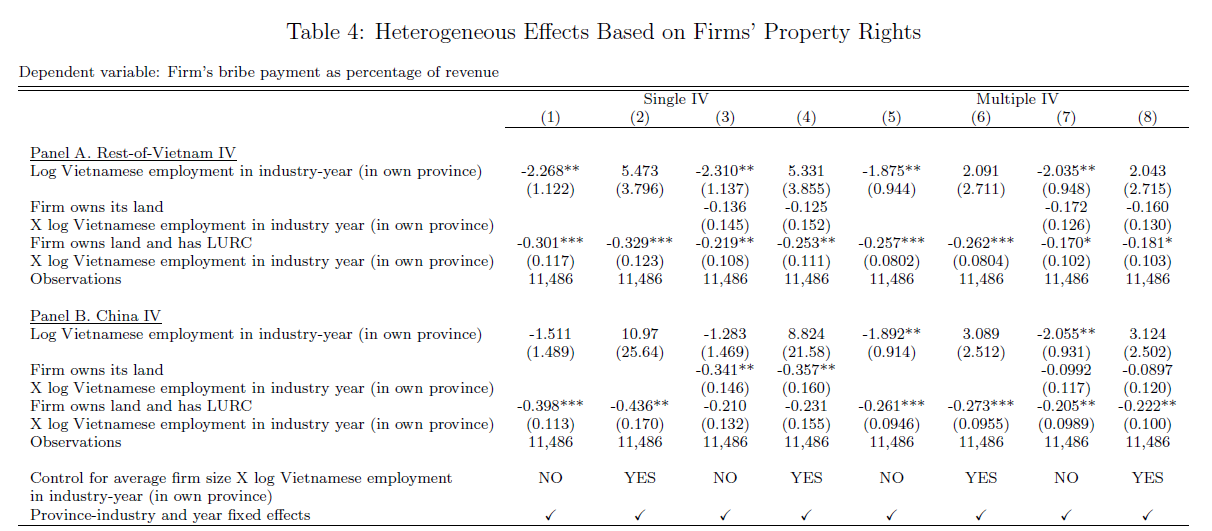
\includegraphics[width=1\linewidth]{12.png}
\end{figure}

\end{frame}
%%%%%%%%%%%%%%%%%%%%%%%%%%%%%%%%%%%%%%%%%%%%%%%%%%%%%%%%%%%%%%%%%%%%%%%%%%%%%%%%%%%%%%%%%%%%%%%

%%%%%%%%%%%%%%%%%%%%%%%%%%%%%%%%%%%%%%%%%%%%%%%%%%%%%%%%%%%%%%%%%%%%%%%%%%%%%%%%%%%%%%%%%%%%%%%
\begin{frame}{Firms operating in multiple provinces}

\begin{figure}
\centering
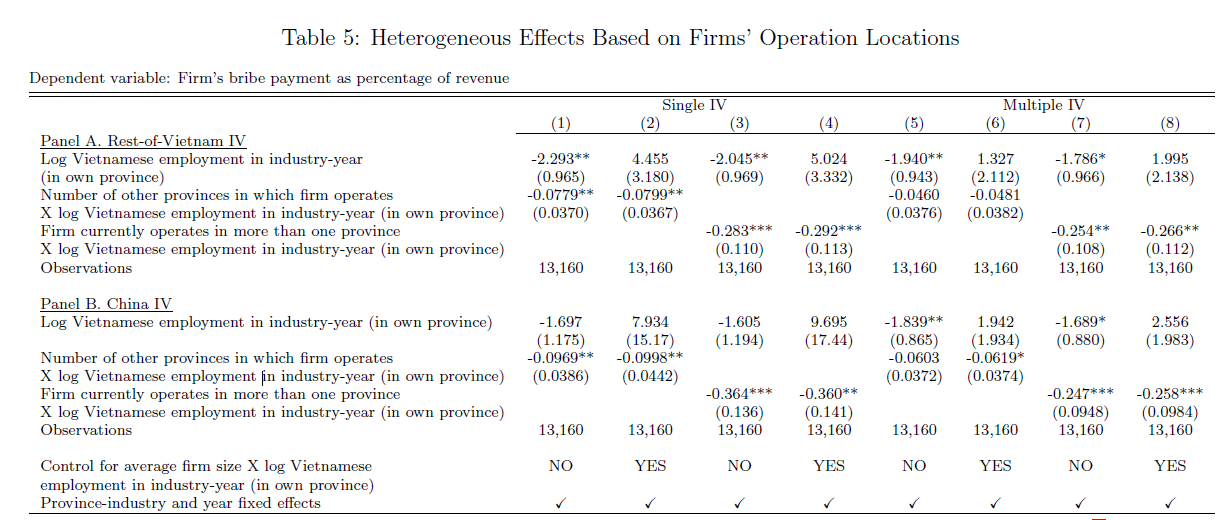
\includegraphics[width=1\linewidth]{13.png}
\end{figure}

\end{frame}
%%%%%%%%%%%%%%%%%%%%%%%%%%%%%%%%%%%%%%%%%%%%%%%%%%%%%%%%%%%%%%%%%%%%%%%%%%%%%%%%%%%%%%%%%%%%%%%

%%%%%%%%%%%%%%%%%%%%%%%%%%%%%%%%%%%%%%%%%%%%%%%%%%%%%%%%%%%%%%%%%%%%%%%%%%%%%%%%%%%%%%%%%%%%%%%
\section{Conclusion}
%%%%%%%%%%%%%%%%%%%%%%%%%%%%%%%%%%%%%%%%%%%%%%%%%%%%%%%%%%%%%%%%%%%%%%%%%%%%%%%%%%%%%%%%%%%%%%%

%%%%%%%%%%%%%%%%%%%%%%%%%%%%%%%%%%%%%%%%%%%%%%%%%%%%%%%%%%%%%%%%%%%%%%%%%%%%%%%%%%%%%%%%%%%%%%%
\begin{frame}{Conclusion}

\begin{itemize}
\item Establishes two empirical facts:
\begin{enumerate}
\item Economic growth (as measured by industry-level employment growth) reduces the proportion of rm revenues extracted by government officials as bribes.
\item This reduction in corruption is larger for firms that can more easily relocate.\\~
\end{enumerate}

\item These facts map to the two main contributions of the paper:
\begin{enumerate}
\item An important empirical contribution: Despite much interest in the relationship between corruption and growth, we provide some of the first rigorous causal evidence on the effect of growth on corruption.
\item Lay out a mechanism through which economic growth reduces corruption.
\end{enumerate}




\end{itemize}


\end{frame}
%%%%%%%%%%%%%%%%%%%%%%%%%%%%%%%%%%%%%%%%%%%%%%%%%%%%%%%%%%%%%%%%%%%%%%%%%%%%%%%%%%%%%%%%%%%%%%%


















\end{document}
